\documentclass{article}

% if you need to pass options to natbib, use, e.g.:
%     \PassOptionsToPackage{numbers, compress}{natbib}
% before loading neurips_2018

% ready for submission
% \usepackage{neurips_2018}


% to compile a preprint version, e.g., for submission to arXiv, add add the
% [preprint] option:
%     \usepackage[preprint]{neurips_2018}

% to compile a camera-ready version, add the [final] option, e.g.:
\usepackage[final]{nips_2018}

% to avoid loading the natbib package, add option nonatbib:
%     \usepackage[nonatbib]{neurips_2018}

\usepackage[utf8]{inputenc} % allow utf-8 input
\usepackage[T1]{fontenc}    % use 8-bit T1 fonts
\usepackage{hyperref}       % hyperlinks
\usepackage{url}            % simple URL typesetting
\usepackage{booktabs}       % professional-quality tables
\usepackage{amsfonts}       % blackboard math symbols
\usepackage{nicefrac}       % compact symbols for 1/2, etc.
\usepackage{microtype}      % microtypography
\usepackage{bm}
\usepackage{amsmath}
\usepackage{amssymb}
\usepackage{amsthm}
\usepackage{graphicx}
\usepackage{bbold}
\usepackage{graphicx}
\usepackage{xcolor}
\usepackage{soul}
% for writing algorithm table
\usepackage{algorithm,algcompatible,amsmath}

\DeclareMathOperator*{\argmax}{\arg\!\max}% https://tex.stackexchange.com/q/83169/5764
\algnewcommand\INPUT{\item[\textbf{Input:}]}%
\algnewcommand\OUTPUT{\item[\textbf{Output:}]}%

\parindent30pt

\title{Considerations for improving training time and generalization of Deep Reinforcement Learning algorithms for power grid management}

\author{
  Team members: Felipe Buchbinder, Shota Takeshima, Young Kyung Kim
}

\begin{document}
\maketitle

\section*{Abstract}

Electrical power grids are an essential, yet extremely complicated piece of the infrastructure of city life. Various scholars used different reinforcement learning algorithm to train an agent that would make efficient decision. Yet, such agent had limitation as it took more than 4~7 years to train to have better performance compared to baseline model. For this we explored different methods, such as inference and behavior cloning, to shorten the training period. We were not able to shorten the training period with those methods. Therefore, we discussed about how we would use Model Agnostic Meta Learning(MAML) algorithm to shorten the training period.

\section{Introduction}
\label{section:Introduction}

\subsection{Motivation and importance of the problem}
\label{section:motivation}

Electrical power grids are an essential, yet extremely complicated piece of the infrastructure of city life. Responsible for the generating electricity and delivering it to the final consumers, the sheer sizes of some of these power grids are a testimony to the difficulty of managing them. The Synchronous Grid of Continental Europe \cite{SGCE}, for example, provides electricity to over 400 million people in 24 countries. In North America, two power grids are responsible for providing energy to the entire region, with the exception of Texas, Québec and Alaska \cite{NATG}. 

Managing such power grids is as complex as it is relevant. Unexpected fluctuations in supply and demand may lead to power shortages (such as the 2003 Northeast Blackout, that affected an estimated 55 million people in US and Canada \cite{Northeast-Blackout}, or to other adverse effects (such as when clocks in Europe ran slow because Kosovo used more electricity than anticipated as a result of its conflict with Serbia in 2018 \cite{Kosovo}. Human tampering is also another cause for concern, as seen in the California energy crisis, when electricity companies such as Enron deliberately created a shortage in electricity supply in order to inflate prices \cite{California-Energy-Crisis}.

Even when power grids are operating normally, there is still a loss due to the complexities of managing such behemoths. In the U.S., for instance, as much as 5\% of all generated energy is lost before reaching the customers \cite{EIA}, leading states like New York to plan spending US\$30 billion over the next decade in power grid maintenance alone \cite{NYSERDA}. 

Smart grids have been proposed as a mean to manage power grids more efficiently \cite{SmartGrid}. By implementing telemetry across the entire grid and employing algorithms that can seamlessly adjust the generation, transmission and distribution of energy, experts argue we could reduce losses and environmental impact without significant impact to current electricity prices. To be precise, as far as residential and commercial buildings are concerned, estimates are that the CO2 emission of buildings can be reduced by 50-90\% \cite{RLEM2020}.

While plans have been proposed to substitute both the North American \cite{SmartGrid-USA} and the European \cite{SmartGrid-EU} current power systems by smart grids, actually implementing smart grids, however, has caveats and challenges of its own. Among the challenges, one that is of particular concern to Artificial Intelligence (AI) scholars is how to train the algorithm that will manage such grids. In this paper, we use Reinforcement Learning to train an agent to manage a small power grid generated by the City Learn simulator package \cite{Vazquez-Canteli2019}. We use this as an instance to illustrate how training times may be too long to be practically feasible, thereby compromising the potential values of such agents in real-world applications. We further discuss alternatives to speed up the training process.

\section{Literature Review}
\subsection{General statement of the Reinforcement Learning problem}

Reinforcement Learning (RL) is one of the branches of Machine Learning (ML), alongside with Supervised and Unsupervised Learning. In RL, there is an agent and an environment. The agent observes certain features of the environment and takes actions from what it observe. As a result of the action it takes, it receives a certain reward from the environment and changes the environment in some way. It then observes certain features of this new environment, and takes a new action. As a result, he gets a new reward and the environment is changed again. Thus the agent takes a succession of \emph{actions} based on what it perceives as being the \emph{state} of the environment, and receives a \emph{reward} for each action. The goal of RL is to teach the agent how to act in order to maximize the expected value of the reward it could earn. Two terms are important in this statement: "teach how to act" and "expected value."

By "teach the agent how to act", we mean deciding which action to take for each observed state of the environment. This is called a \emph{policy} and do not need to be deterministic: one may perfectly well have a policy that states that, when faced with an environment in a certain state, the agent should randomly pick an action from a given probability distribution defined over the set of admissible actions. Ultimately, the "answer" for a Reinforcement Learning problem is a certain policy i.e. a function that connects each state in the environment, either to an action to be taken (if the policy is deterministic) or to a probability distribution from which the action is to be drawn (if the policy is stochastic).

By "expected value value", we mean the exact same thing that is meant in finance by the homonymous expression. Namely, that imminent rewards are perceived as more valuable than similar rewards in a distant future, so we apply a \emph{discount factor} for every period we have to wait in order to perceive a reward. Imminent rewards are more valuable because rewards in a distant future have a lot of risk as there might unexpected obstacles in future that decrease the reward. As a result, the values of rewards decrease exponentially with the time we have to wait to perceive them.

If we were to combine all these ideas into a single mathematical expression, we could state that the goal of RL is to solve the following problem, given a set of problem-specific initial conditions and constraints:

$$
\pi^*=\arg \max_{\pi} \mathbb{E}_\pi \left[ \sum_{t=0}^{+\infty} \gamma^t r(s_t,a_t) \right ] \label{1}
$$

Here, $\gamma$ is the discount factor and  $r(s_t,a_t)$ is the reward obtained at time $t$ as a result of taking the action ($a_t$)  prescribed by policy $\pi$ given the state ($s_t$) the agent finds itself at that time. The reader may recognize the term within the square brackets as the present value of a cash flow of rewards. But since the policy is arguably stochastic, there is uncertainty on the exact course of action to be followed and therefore on the rewards to be perceived. Thus we cannot maximize the present value of expected rewards, but only its expected value given the policy the agent undertakes. Our goal is to find the policy that maximizes such expected value.

In particular, if $\gamma \to 0$, our policy consists on choosing what is the immediate best solution, with no regards for what might happen in future time steps. It's a greedy policy. Conversely, with $\gamma\to1$, no discounting is in place, and similar rewards are perceived as having equal values regardless on how much the agent has to wait in order to perceive them.

Furthermore, note that no mention is made as to how the environment moves from one state to another, or the probabilities with which states succeed each other. All that is necessary is to observe the rewards that result from following the prescribed policy. In this sense, RL is\emph{model free}. This is an advantage of RL for real life problems, where we are often ignorant on how the real world works, and are only conscious of our actions and their consequences. This is, in a way, quite poetic. There is no blueprint to life. We learn by doing. By acting, and facing the consequences of our actions. That's how RL works, and that's a feature that makes it very applicable to so many real-life problems.

In addition, states need not be perfectly observed. Thus, in the first paragraphs of this section, we were careful in our choice of words, when we said  that "agent observes certain features of the environment and acts on what he observes". The agent does not need to observe \emph{all} features of the environment. But whatever it does observe, that's what it acts upon. Our agent will try to find the best actions it can, given the information it has, however partial or noisy they may be. The fact that information may not be neither complete nor perfect is very realistic, and accounts for another advantage of RL over other ML approaches such as Supervised or Unsupervised Learning, which are much more silent about these issues.

\subsection{Overview of heuristics for solving the Reinforcement Learning Problem}

So how does one go about solving Equation $\ref{1}$?

There are essentially two ways to do this: one can either follow a \emph{value-based approach} or a \emph{policy-based approach}.

In a \emph{value-based approach}, one tries to determine the value of taking each possible action on each possible state. By value we mean the expected value in Equation $\ref{1}$ i.e. the thing which we want to maximize. If an agent knows the value of taking each possible action on each possible state, it can easily figure out the best action to take in whichever state it happens to be in. All it has to do is pick whichever action moves it to the next state of highest value.

In more mathematical terms, in the value-based approach, one has to discover a function $Q: \mathcal{S} \times \mathcal{A} \to \mathbb{R}$ that associates the value of taking a given action $a \in \mathcal{A}$ when in state $s \in \mathcal{S}$. By value we mean the expected value of all future rewards gained by the agent.

The optimal value of this function will typically be improved at every iteration according to an equation known as the Bellman equation:

$
Q^{new}(s_{t},a_{t}) \leftarrow \underbrace{Q(s_{t},a_{t})}_{\text{old value}} + \underbrace{\alpha}_{\text{learning rate}} \cdot  \overbrace{\bigg( \underbrace{\underbrace{r_{t}}_{\text{reward}} + \underbrace{\gamma}_{\text{discount factor}} \cdot \underbrace{\max_{a}Q(s_{t+1}, a)}_{\text{estimate of optimal future value}}}_{\text{new value (temporal difference target)}} - \underbrace{Q(s_{t},a_{t})}_{\text{old value}} \bigg) }^{\text{temporal difference}}
$

One challenge to this approach arises when the number of states is very large, and in particular, when it is infinite. In this scenarios, some states may only seldom be visited. One way to deal with this is by encoding each state by a finite vector of essential features $\phi$. It's as if, rather than having a list of infinite possible states, we had a small set of features that matter for decision making. Mathematically, this means we move from having an infinite number of possible states, $\{s_0, s_1,s_2...\}$, to having a function $s(\phi)$, which enables us to estimate which state we are in based on a small set of features $\phi$. Since it is impossible to visit an infinite number of states, one must learn how to infer the rewards of each state based on the values of $\phi$ observed for the set of states that actually were visited. This task is often accomplished with Deep Learning techniques.

In a \emph{policy-based approach}, one tries to determine the optimal policy directly, without resorting to the intermediate step of calculating the values of taking each action on each possible state. This is done by expressing the policy as a function $\pi_\theta(a,s)$ that assigns a probability of taking an action $a$ when on a state $s$, and then seeking to find the optimal values of the parameter vector $\theta$. 

\subsection{The Soft Actor-Critic (SAC) algorithm}

Each of these approaches has its strengths and weaknesses. One approach to combine both approaches and thus leverage their strengths is the \emph{actor-critic} algorithm. The "actor" acts following a certain policy. The "critic" observes the rewards it perceives and uses this to calculate the values of each action at each state. These values are then used by the actor to estimate the optimal policy. It then enacts this policy, providing more information for the critic to update its values estimated. And thus, both actor and critic improve their respective performances, until the actor's estimate of the optimal policy converges.

In practice, the actor and the critic are two neural networks. The critic tries to find the function that relates $\phi$ to the rewards perceived at a given state, while the actor tries to find the parameters $\theta$ that lead to the optimal performance $\pi_\theta$. Both neural networks interact and evolve together. This approach of combining neural networks is no novelty to AI literature, and has been successfully implemented in applications such as Generative Adversarial Neural Networks or Variational Autoencoders.

The actor-critic algorithm can be improved by fostering exploration. In all RL algorithms, there is an inherent concern over how to balance exploration and exploitation. The latter (exploitation) consists of taking those actions that are already known to perform the best, while the former (exploration) consists of attempting actions which may seem senseless on the hopes that they may help us discover a better policy than the one we currently have. No learning is possible without some degree of exploration. Yet, since exploration leads to failure much more often than it leads to success, it's easy to overlook it. This is especially striking in continuous spaces of action, where the probability of exploring any given specific action tends to zero, as does the probability of that specific action being the jackpot. So how can we encourage an agent to explore new courses of action on a continuous-space of possible actions?

The \emph{soft-actor-critic} (SAC) algorithm does that by adding an additional term to the traditional RL objective function. This function is (proportional to) the entropy of the policy. Hence, it praises policies which acknowledge doubt on to what is the best course of action to pursue, and punishes policies that are overly confident that only one specific action can be taken in any  given case. Under this framework, Equation $\ref{1}$ becomes:

$$
\pi^*=\arg \max_{\theta} \mathbb{E}_{\pi(\theta)} \left[ \sum_{t=0}^{+\infty} \gamma^t r(s_t(\phi),a_t) + \alpha \mathcal{H_\pi}\right ] \label{2}
$$

where $\mathcal{H_\pi}$ is the entropy of policy $\pi$, now parametrized in terms of $\theta$, and $\alpha$ is a measure of how much one wishes to penalize a policy for failing to explore. The critic will try to arrive at the value of $\phi$ best estimates  $Q_\pi(s,a)=\sum_{t=0}^{+\infty}r(s_t(\phi),a_t)$, while the actor will attempt to find the value of $\theta$ that produces the optimal policy. Note that $Q_\pi(s,a)$, the function estimated by the critic, is dependent on $\pi$, the policy provided by the actor. Conversely,  $\pi^*$, the policy that the actor believes to be optimal, is dependent on $Q_\pi(s,a)$, the function estimated by the critic.

\subsection{Imitation Learning}

There is yet another way to solve the Reinforcement Learning that evades solving equation $\ref{1}$ altogether. Rather than letting a computer figure out the best policy by acting and suffering the consequences of its actions, why not teach the computer simply to copy the behavior of someone who already knows what to do?

The task therefore becomes to find out what would an "expert" do in \emph{every} situation given that we have a dataset of what he said should be done in \emph{some} situations. The "expert" behavior thus becomes a target, and our goal is to find a predictor for it. Our reinforcement learning problem is thus reduced to a classical supervised learning problem \cite{rashidinejad2021}.

Granted, the performance of the trained algorithm will be upper bounded by the performance of the expert. Such caveat notwithstanding, this approach is very convenient when an "expert" is easily available, and when quantifying the rewards of each action is difficult \cite{smartlab2021}. In other words, imitation learning is useful when it is easier for an expert to show what must be done than to actually figure out the rewards for each possible action.

Such is the case, for example, on autonomous cars \cite{pomerleau-2021}. One can easily find a driver and observe that he signals a left turn before actually turning left. Quantifying the reward obtained by such signalling, however, is much harder.

Another advantage of imitation learning is that it draws upon algorithms from classical supervised learning, which tend to be much more simpler and faster to run than those of RL.

A downside of using classical supervised learning algorithms, however, is that these algorithms often suppose that training samples are independent. This is seldom the case. In the self-driving car example, what the driver sees in one moment cannot be said to be independent from what he will see in the following moment. Quite on the contrary, the latter is a direct consequence of the actions taken by him on the former. By treating observations as independent, errors committed in one circumstance add up, leading the algorithm to learn a behavior that may ultimately be very different than what the expert would actually do \cite{rashidinejad2021}.

\subsection{Inference}

Suppose we want to create an agent that learns how to manage a power grid in New York. Suppose we already have such an agent, but it has actually learnt how to manage the power grid in London, not in New York. Anyone faced with this situation will be tempted to get the same algorithm that has been working in London and apply it in New York. Yes, the climates are different, so we would expect the agent's performance in New York to be inferior than the agent's performance in London. Still, given the great time it takes to train an agent from scratch, copying the agent from London seems like an economically sensible solution. This is called \emph{inference}.

If the agent were copied from London to New York and then continued to be trained on New York, this would be called \emph{transfer learning}.

If, however, the agent did all its learning in London and then were merely applied to New York (with no further learning there), this would be called inference.

It is expected (but not mathematically necessary) that the agent's performance on the second location will be inferior to the performance on the first location, though this may change with further learning. Moreover, it is reasonable that the change in performances observed in both contexts should increase with the dissimilarity between such contexts. Thus, copying an agent from London to New York shouldn't entail a dramatic a drop in performance as copying it from London to Nairobi.

In this paper, as we shall further explain, we consider 4 different climate zones, and employ agents trained in one zone to act on another.

\subsection{Rule-Based Control}

Rule-based control (RBC) consists on having an agent act according to a set of rules that he is given. Technically, it doesn't qualify as machine learning, let alone as reinforcement learning. Yet, precisely for not qualifying as machine learning, it serves as a noteworthy benchmark as to the gains that can be achieved by proper Machine Learning algorithms.

Whereas in ML a decision rule is derived from the data, in RBC the decision rule is explicitly given to the machine. Such rule may be derived from expert knowledge, that is, from human knowledge. Or it can be even simpler than that.

In the case of a power grid management, for example, an RBC approach might be to never stock any energy for future use, and just use energy from the grid, however much it costs. Alternatively, the rule could be to stock energy for future use when its price is less than a certain threshold value. The key point is that these rules are given, not learned. Thus, for being the quintessential opposite of ML, RBC serves as an interesting benchmark as to whether the machine has learned anything at all.

Having reviewed the field of RL from a general point of view, we now present the simulator we will be using for this paper. Subsequently, we will delve into how extant literature has employed RL to tackle the challenges of power grid management and, in particular, to address the issue of demand response.

\subsection{The City Learn power grid simulator}

City Learn \cite{Vazquez-Canteli2019} is a simulation environment for energy demand response. In its simplest form, it considers a generator (that supplies energy) and a building (that consumes energy). Demand for energy varies according to time zone, time of day, and types of buildings. The building can stock energy during periods of low-demand to use during periods of high-demand, but there's a limit to how much energy the building can stock. The building seeks to minimize a cost function which considers a series of factors: amount spent on energy, risk of shortage, risk of rampage, and others.

In a not-so-simple scenario, there are multiple generators and multiple buildings. An agent decides how much energy should be used by or stocked at each building, so as to minimize the cost function for the \emph{network} (not any individual building). There are various different types of energy that can be considered, such as thermal energy, batteries, and air-to-water heat pumps. While they can all be stocked, they do have different prices.

To be more specific, City Learn simulates an environment where a set of $N$ buildings are, at any given time $t$, in a state that is completely defined by 28 variables. These variables are of the following types:

\begin{itemize}
\item Temporal variables as “month”, “day”, or “hour”
\item Temperature variables
\item Humidity variables
\item Diffuse solar radiation variables
\item Storage variables(How much energy is stored)
\end{itemize}

We find it important to highlight that all but the last type of variable are related to the demand of energy. Indeed, the demand for energy varies through time depending on temperature , humidity or the speed with which energy dissipates. The last kind of variable, however, refers to storage. And storage is ultimately a "managerial" decision: it's how the agent chooses to manage the network. Such choice has implications that deserve our attention: If a building stocks energy today, it is betting that energy today will be cheaper than in the future. Moreover, if it chooses to use energy it has previously stocked, it is limited by the choice of how much it decided to stock in the past. Hence, the storage variables insert a path dependency into our problem.

As for the actions, there are only 2 actions possible for the agent to take

\begin{itemize}
\item Increasing or decreasing the energy in cooling storage
\item Increasing or decreasing the energy in domestic hot water storage
\end{itemize}

Since each building has its own storage, such 2 actions are, in reality, 2 actions \emph{per building}. In other words, the agent must decide how much energy will put in storage (or taken out of storage) for each building.

Such agent may be a single agent, managing the entire network, or a set of agents, one responsible for each building, which act independently but can communicate with each other.

Having presented both the field of RL and the simulator we will employ, we now proceed to discuss how RL scholars have previously addressed the issue of power grid management. We shall be particularly concerned with a particular problem in power grid management (namely, demand response) for which we will give a precise definition in the upcoming section. Finally, we will show how this present paper articulates itself with extant literature, and how it relates to the ongoing debate on how can RL be used to improve current practices of power grid management. 

\subsection{Reinforcement Learning for demand response}

The task of managing a power grid conforms well to the basic tenants of RL. For each action one takes on a power grid, one has a corresponding consequence to either enjoy or suffer. The grid can have a myriad of different states and unknown transition probabilities. In short, one must teach an agent which actions to take given only the rewards of such actions. That's the quintessential example of RL \cite{Lambert2020}. Indeed, there is a vast literature on employing RL to managing power grids (e.g. \cite{Ademoye2012, Hadidi2013, Glavic2017, Mocanu2019}).

Glavic (\cite{Glavic2017}) performed a literature review where he analyzed extant challenges and concerns about the employment of RL to power grid management concluding the overall sentiment in the scientific community is that RL is a very promising approach to deal with the task at hand.

Indeed, RL has been employed to multiple problems, all of which fall under the general category of power grid management. Thus, some authors focus on optimizing the generation of electricity (e.g. \cite{Wang2016}), others focus on its distribution \cite{Gemine2017}, while others focus on managing the consumption of energy itself \cite{Xu2020, Mocanu2019, Si2021}. Likewise, some authors focus on controlling the power grid \cite{Yousefian2016}, others in stabilizing it \cite{Hadidi2013}, while others attempt to modulate demand by setting energy prices dynamically \cite{Tsui2012}.

This latter stream of research, in particular, has been receiving a significant share of scholarly attention, and even has a name of its own: demand response. Demand response consists of managing the power grid by modulating the demand for energy. This will typically be done by some sort of price incentive, lowering energy prices when one wishes to increase demand, and raising energy prices when one wishes to decrease it \cite{Christensen2020, Kurte2020}. Our paper falls into this category. 

We consider the problem of a small power grid to which buildings of different kinds are connected. The price of electricity varies with time and, in particular, it increases as a response to an unexpected ramping in demand. Buildings use electricity to either heat up or cool down, thereby maintaining a pleasant temperature. The need to heat up or cool down is determined by the outside temperature which varies throughout the year in a way that is specific to the climate zone where the power grid is located. Buildings have the option to store either hot or cold water, that can be used to either heat up or cool down the building at some later time. Hence, if a building is anticipating hot weather on the upcoming days and the price of electricity is cheap at present, it may wish to store cold water, so it can cool itself down when the temperature rises and energy prices are no longer cheap. All data is simulated, and we use the City Learn package to this end.

%In making such decisions, however, we assume buildings act independently to each other, with no information sharing between them.(I just pulled it out, as there is a information sharing part)

Unlike supervised and unsupervised learning, RL often makes use of simulated data (with some exceptions e.g. \cite{Xu2020}). Kang \cite{Kang2019} notes that one reason for the ubiquity of simulated data on RL research is because RL requires copious amounts of data, to the extent where getting such data might be very costly, if at all feasible.  Beattie \emph{et al.} \cite{DeepMind2021} make an interesting remark on this point. They argue that, in some real-world application domains, data may be generated slowly. This is, indeed, the case with our paper. In order to learn how to efficiently manage  energy throughout yearly cycles of succeeding seasons, one would need many years of data. By using simulations, such data can be obtained with no need to wait. 

There is, of course, a trade-off here. While simulated data is much faster and cheaper to obtain in large amounts, it may fail to accurately replicate what real-data would look like. In plain terms, one can always cast doubt on whether a simulator is indeed realistic \cite{Dulac2019}. This has led some researchers to endeavor to combine real-data and simulated data (\cite{Kang2019, Hanna2019, Mocanu2019}). 

In spite of such promising developments in the field, there has been a remarkable development in simulators targeted at RL research (e.g. \cite{DeepMind2021, OpenAIGym}). At present, most research on RL relies on simulated data. Our paper follows this tradition, and uses the City Learn simulator \cite{Vazquez-Canteli2019}.

The City Learn simulator simulates a small power grid network. As concerns its size, our grid is an intermediate between the one modelled by Kuznetsova \emph{et al.} \cite{Kuznetsova2013} (which consists of a consumer, a generator and a battery for storage), and the one modelled by Yousefian and Kamalasadan \cite{Yousefian2016} (where dispersion over a large area is a feature that must be considered). In our power grid, there are multiple buildings, but they are sufficiently close together for delays between generation and consumption to be neglected. 

In addition, we have multiple buildings and pay no attention to how is energy distributed inside a building. In this respect, our paper is opposite to that of Tsui and Chan \cite{Tsui2012}, where one considers a single home but worries about the multiple appliances it contains. 

It is important to highlight, however, that 9 different types of buildings are considered. This should arguably enhance the adherence of our simulated power grid to reality, since in the real-world, there exists buildings with different demands for energy. A commercial building has high demand for electricity during work hours, but a smaller demand during the weekend. The opposite is true for residential buildings.  

Likewise, we consider 5 different climate zones, which means there are 5 distinct ways to simulate how temperature (and hence energy demand) evolves throughout the year. 

In our simulator, buildings can use energy to store either warm or cold water, that will subsequently be used for cooling or heating. Scholars such as Tsui and Chan \cite{Tsui2012} and Xu \emph{et al.} \cite{Xu2020} allow for many more uses of electricity within a building, but their interest lies on a single household. Conversely, scholars such as Ademoye and Feliachi \cite{Ademoye2012} and Mocanu \emph{et al.} \cite{Mocanu2019} deal with the energy demand as a black box, with no distinction whatsoever as regards its use. Our paper strikes a balance between both approaches: while not delving into all the possible uses of electricity within a building, by allowing two possible uses, it acknowledges that this utility may be used in different ways.

In addition, it's worthy to note that buildings can only store or use energy. They cannot generate energy. In this regard, our approach differs from Wang \emph{et al.} \cite{Wang2016}, where buildings are equipped with photovoltaic generating systems. This should arguably increase the need for energy storage. While data from the International Energy Agency \cite{IEA2020} suggests global photovoltaic capacity has been doubling every 2.4 years, the same report shows that such capacity is capable of meeting only 3\% of the global demand for energy. Hence, at present, it is more realistic to suppose buildings do not have the ability to generate their own energy than to suppose otherwise.

When all such buildings are brought together and integrated into a power grid, one must make the decision as to how such grid is to be managed. One possibility, for example, is to have a single agent decide how each building should act, so as to minimize the cost of managing the entire grid. Such an agent would need to have information on each building's energy needs and storage levels. In its own turn, the agent would combine all this information into a single objective function that considered the costs of all buildings, thus achieving what Economic literature calls the social optimum. Yousefian and Kamalasadan \cite{Yousefian2016} is an example of such an implementation. 

One practical problem of the single agent approach is that granting its information on the energy consumption of each individual building may be perceived as a violation of privacy rights. Moreover, granting control over the power grid to a single agent raises concerns over malpractices such as observed during the California Energy Crisis \cite{California-Energy-Crisis}. Finally, minimizing the collective cost of energy doesn't necessarily guarantee that each individual building will have its own cost minimized, which may also pose an issue in more individualistic societies. 

Another possibility as to how to manage a power grid is to do precisely the opposite: have each building decide on its own how much energy to use or to store. In plain terms, rather than having a single agent decide what everyone should do, each building shall decide for itself. In this multi-agent approach, each building optimizes its own objective function. In principle, nothing precludes buildings from sharing information among themselves, so it is still possible to incorporate information from multiple buildings within each objective function. Still, since each building optimizes its own objective function (possibly conditioned on its expected behavior of the remaining buildings), there is no guarantee that a social optimum will be achieved. Nonetheless, concerns over privacy, excessive market power and the limitation of the individual's freedom to chose have been greatly reduced. Li \emph {et al.} \cite{Li2012}, Dhamankar \emph{et al.} \cite{Dhamankar2020}, Xu \emph{et al.} \cite{Xu2020} and Ademoye and Feliachi \cite{Ademoye2012} are examples of this approach.

In our paper, we use a multi-agent approach with no information sharing. This means each building maximizes its own objective function, with no regards whatsoever for other buildings. We chose a multi-agent approach because, in our understanding, it is more realistic, as it evades the caveats cited previously. In addition, by doing so, we align ourselves with the majority of previous research. A third, but equally important reason, results from a meeting we had with the developer of the City Learn simulator, in which he suggested we used the multi-agent approach, since its code is more stable, and has been more tested, than the single agent.

In reality, a hybrid model is often observed, where a large network is broken into regions and, within each region, the generation, transmission and distribution of energy are managed by a single-agent fashion, whereas the buildings are granted autonomy to decide for themselves how much to consume or store. In other words, within a certain region, the decisions pertaining generation, transmission and distribution are made by centralized agents, whereas the actual consumption of energy is made by decentralized agents. The Synchronous grid of Continental Europe \cite{SGCE}, for example, is managed by the European Network of Transmission System Operators for Electricity (ENTSO-E), an organization that is, in turn, comprised by 42 other organizations (called Transmission System Operators, or TSOs) that manage the generation, transmission and distribution of electricity within specific regions of the grid. Since the entry costs of generation, transmission and distribution are formidably high, these activities are natural monopolies, so concerns over market power of TSOs cannot be solved by competition. Thus, a single agent approach lends itself naturally to this scenario. The same cannot be said, however, for the demand side of the grid. Hence, as far as buildings are concerned, they are autonomous to make their own decisions regarding energy consumption. Here, what we have is a multiple-agent approach. We have been unable to find any papers that employ such a hybrid model of power grid management. While we acknowledge that such vacuity may be a result of the increased complexity of a hybrid model, we should also point out that this is (to the best of our knowledge) an open field for future research.

\section{Data}

\subsection{Simulator}
CityLearn is an OpenAI Gym environment for the easy implementation of RL agents in a multi-agent demand response setting to reshape the aggregated curve of electrical demand by controlling the energy storage of a diverse set of buildings \cite{CityLearn}. Its main objective is to facilitate and standardize the evaluation of RL agents such that it enables benchmarking of different algorithms. CityLearn includes energy models of air-to-water heat pumps, electric heaters, and the pre-computed energy loads of the buildings, which include space cooling, dehumidification, appliances, domestic hot water (DHW), and solar generation. We try to implement a new reinforcement algorithm (RL) into CityLearn to control the storage of DHW and chilled water. The RL agents send their control actions hourly and receive a set of states and rewards in return. Indoor temperatures in the buildings do not change, as the environment automatically constraints the actions of the controllers and ensures that the energy supply devices are large enough to guarantee that the energy demand of the buildings is always supplied. The RL agents can decide how much cooling or heating energy store or release at any given time. A backup controller integrated in CityLearn guarantees that the energy supply devices prioritize satisfying the energy demand of the building before storing any additional energy. The simulator allows us to configure the building properties and their number to be controlled by the agent(s). In addition, it also provides four climate zone setting to evaluate if the agent can works generally in several environments. As Figure \ref{fig:ave_tmp_by_cz} shows, the climate properties, such as temperature inside/outside the buildings differ by the climate zone.

\begin{figure}[h!]
  \centering
  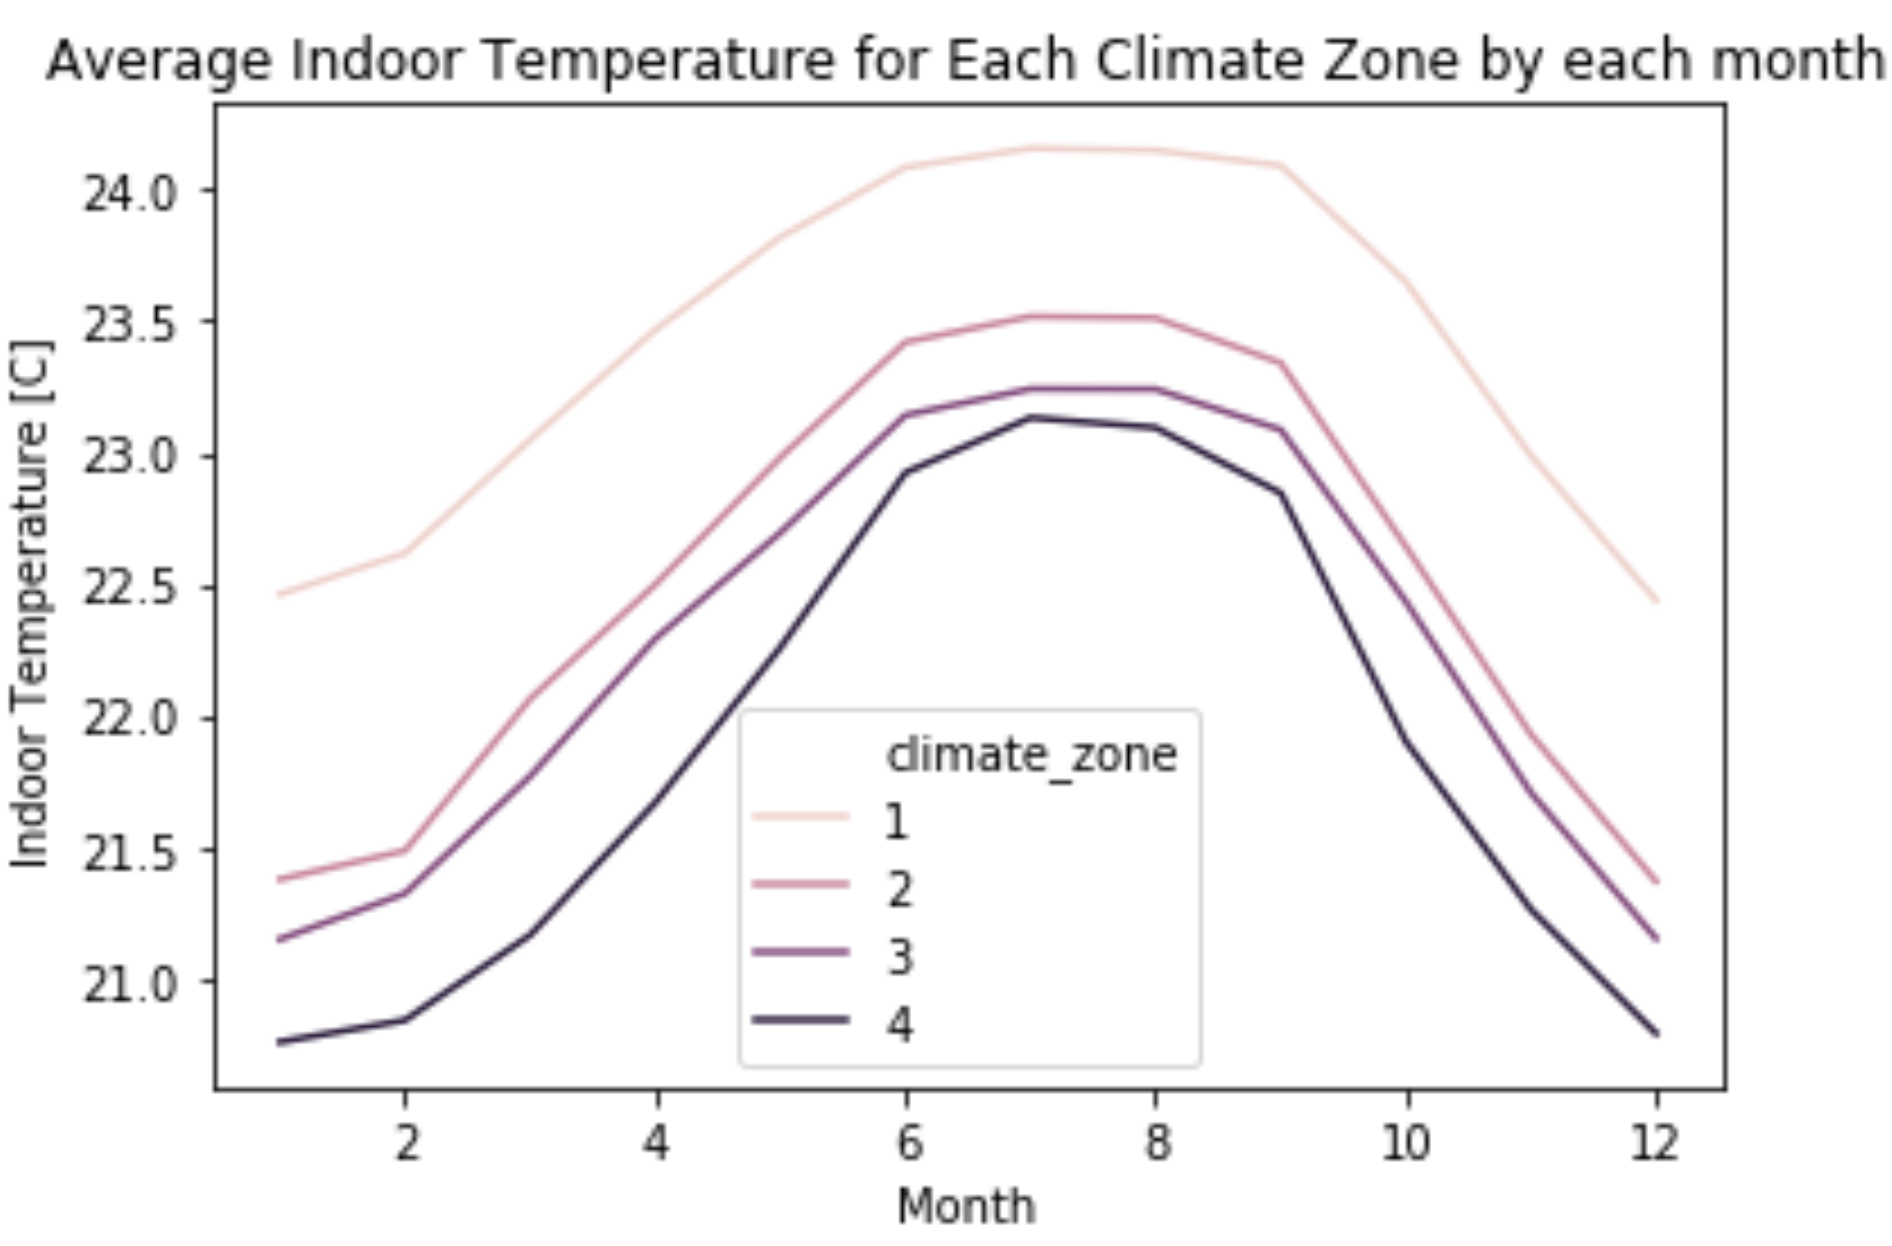
\includegraphics[scale = 0.3]{figures/temp_by_climate_zone.png}
  \caption{Average indoor temperature setting by climate zone}
  \label{fig:ave_tmp_by_cz}
\end{figure}

\subsection{State, reward, and action for reinforcement learning agent}
\label{sec:sra}
% \newline
% - Describe about different parameters for the environment(for example explain about region
% parameter)
% - Describe who is the agent. Describe what are the possible actions. Describe how is reward calculated. 
% \newline
% - Detail number of simulations (and parameters) actually employed. Brief descriptive statistics
% \newline
% - if possible, could you introduce that rule-based controller (RBC) is included in CityLearn as well as how RBC works. by Shota 
% - as well as cost

City Learn simulates an environment where a set of N buildings are, at any given time t, in a state that is completely defined by 28 variables. These variables are of the following types:
\begin{itemize}
\item Temporal variables as “month”, “day”, or “hour”
\item Temperature variables
\item Humidity variables
\item Diffuse solar radiation variables
\item Storage variables(How much energy is stored)
\end{itemize}
\newline

We find it important to highlight that all but the last type of variables are related to the demand for energy. Indeed, the demand for energy varies through time, with temperature, humidity, or with the speed with which energy dissipates. The last kind of variable, however, refers to storage. And storage is ultimately a “managerial” decision: it’s how the agent chooses to manage the network. Such choice has implications that deserve our attention: If a building stocks energy today, it is betting that energy today will be cheaper than in the future. Moreover, if it chooses to use the energy it has previously stocked, it is limited by the choice of how much it decided to stock in the past. Hence, the storage variables insert a path dependency on our problem.
As for the actions, there are only 2 actions possible for the agent to take - Increasing or decreasing the energy in cooling storage - Increasing or decreasing the energy in domestic hot water storage since each building has its own storage, such 2 actions are, in reality, 2 actions per building. In other words, the agent must decide how much energy will de put in storage (or taken out of storage) for each building. Such a central agent may be a single agent, managing the entire network, or a set of agents, one responsible for each building, which acts independently but can communicate with each other. We have considered a set of one agent per building acting independently. For simplicity, however, we often refer to these agents in a singular form.


\section{Methods and Experimental results}
% rewrite our objective to use the methods here
As we mentioned in \ref{section:motivation}, our objectives are reducing the training time while having an appropriate performance for actual real-world use. The baseline performance is calculated by RBC, and our evaluation metric, $cost$, is calculated by comparing with RBC result. Fig \ref{fig:replication_result} shows a training curves of agents trained in climate zone 1 and 4. As the figure shows, after 4-year and 7-year simulations for climate zone 1 and 4 respectively, the agents can produce better operations than RBC's one. Therefore, if energy management by this reinforcement learning technique is required in another climate zone, it might take another at least 4 year to train its agent, which is not an efficient approach. In this section, we introduce two methods we considered to reduce the training time. One is inference approach and another one is behavior cloning. In those subsections, we mention how they work and show the experimental results. Then, we discuss the strengths and weaknesses of each approach.

\begin{figure}[h!]
\centering
\label{fig:replication_result}
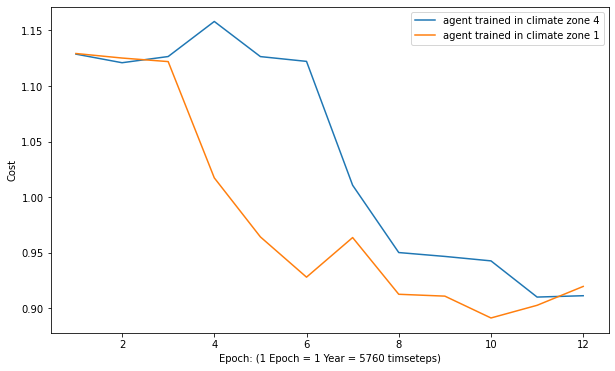
\includegraphics[scale=0.4]{figures/replication_result.png}
\caption{Training curves of agents trained in climate zone 1 and 4}
\end{figure}

\subsection{Inference}
\label{sec:TL}
Reinforcement learning made remarkable advancement in past few years. However, reinforcement learning still faces few difficulties such as the exploration and exploitation dilemma.\cite{zhu2021transfer} The exploitation of knowledge about the environment to improve an agent's performance can start after the agent explored sufficiently enough. For example, one of the reasons the training time is too long to adopt as a real-world application is SAC agent needs to explore about three years to gather enough states and actions for its replay buffer. After exploration, it starts to update weights of its policy and value function networks. As a result, inference, which is an approach to take advantage of external expertise from other tasks to apply into target task, is extremely efficient as it does not require any training or exploration.

In our research, we trained a policy through minimizing $cost$ in a particular climate zone. Also, we assume environments, CityLearn simulator, has the same number and types of buildings in all climate zone. Let $\{Z_s, Z_t\} \in Z$ be environment of the source domain and target domain respectively.

\begin{equation}
\label{eq:opt_policy}
    \pi^* = \argmax_\pi \mathrm{E}_{s \sim \mu_0, a \sim \pi}\left[ Q^\pi_Z(s, a)\right]\\
\end{equation}

% comment: explanation of Q-function is needed. is it in previous section?
where $\mu_0$ is the set of initial states. $a \in A, s \in S$ denotes an action the agent can take and a state from CityLearn simulate in a particular climate, $Z$, respectively. The policy $\pi$ can be described by 

\begin{equation}
\label{eq:policy_func}
    \pi = \phi(D_s \sim Z_s, D_t \sim Z_t): S_t \rightarrow A_t
\end{equation}

In terms of $\phi$, we use a deep neural network as a policy network. Regarding our objective with policy, we aim to find $\pi^*$ for the target climate zone, $ Z_t $ minimizing $|D_t|$ that is the training time in the target climate zone. Concisely saying, we use pre-trained policy and value function network (critic) trained on $Z_s$ and evaluate on $Z_t$ to see how well it performs.

We evaluate how an agent trained in a specific climate zone for 12 years simulation works in another climate zone. Fig. \ref{fig:transfer_learning_result} shows experimental results that how an agent trained on climate zone 1 performs on the target climate zone 4 and vice versa. Costs obtained by policy from zone that it has trained on and from zone that it is has evaluated on are less than 1.0 in both case of climate zone 1 and 4. They are appropriate costs compared to RBC's ones. Hence, we can mention that while originally it takes 12-years to train the agents, inference is an efficient method as it still provide appropriate costs compared to RBC. On the other hand, we can confirm the difference of costs between ordinary learning and inference, which arise from generalization problem. All climate zones CityLearn simulator provides are in the U.S. Hence, there is a possibility that inference makes a larger difference if the source climate zone has no similarity to the target climate zone, especially in actual use. Therefore, as an improvement of this approach, generalization of reinforcement learning is required. It means generating an agent that provides an averagely appropriate cost on any other climate zone and transferring its policy and value function networks.

\begin{figure}[htbp!]
\centering
\label{fig:transfer_learning_result}
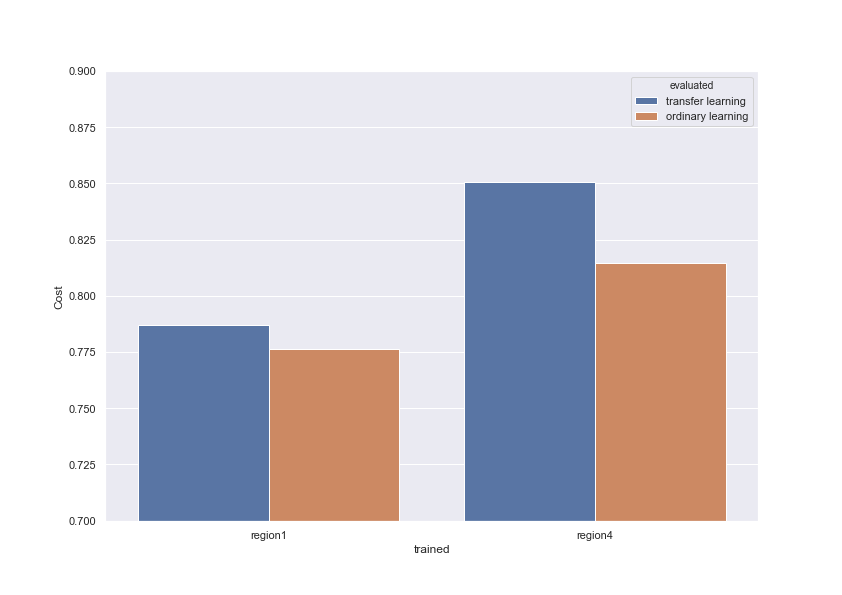
\includegraphics[scale=0.3]{figures/transfer_learning_result.png}
\caption{Comparison of costs obtained after 12-year training and transfer learning}
\end{figure}

\subsection{Behavior Cloning}
In the previous section, \ref{sec:TL}, we can shorten the training time using the inference technique, and simultaneously we concluded that the generalization of the inference approach is necessary, especially for climate zones that have less similarity to the climate zone on which the original agent has trained on. In this section, similarly to the inference, we consider using a policy network that mimics RBC. As we introduced in \ref{sec:sra}, it calculates policy deterministically based on given state variables. Our idea is if an agent has can imitate RBC using deep reinforcement learning algorithm, our agent can generate a cost that is close to 1.0 without no training. Then, we can train additionally to adapt to each climate zone. It is noteworthy that RBC is one of the generalized agents, and it can produce a cost that is 1.0 on every climate zone because it is a baseline to calculate cost itself.

In \textbf{Algorithm\ref{algo:bc}}, the algorithm of behavior cloning is written. First, we gather RBC's demonstrations by letting RBC interact with the target environment. In this process, a pair of state and RBC's actions is appended into the demonstration dataset. Using the demonstration dataset, the policy network extracted from the deep reinforce learning agent is trained. As the algorithm shows, it is trained in a supervised learning manner, and after convergence, the trained network is obtained.

\begin{algorithm}
    \caption{Behavior Cloning}
    \label{algo:bc}
  \begin{algorithmic}[1]
    \REQUIRE $Z:$ environment of the target climate zone
    \REQUIRE $f, \theta:$ policy network and its weights of deep reinforcement learning agent
    \REQUIRE $L, \alpha:$ loss function and step size parameter for update
    \STATE interact RBC with $Z$ and store (s, a) into expert data $D$
    \WHILE{stopping criterion not met}
        \STATE Sample a minibatch of $b$ examples from $D$, ${s_1, \cdots, s_b}$ with corresponding actions $a_i$
        \STATE Compute gradient estimate: $\hat{g} = +\frac{1}{b}\nabla_\theta \sum_i L(f(s_i;\theta), a_i)$
        \STATE Update: $\theta = \theta - \alpha \hat{g}$
    \ENDWHILE
  \end{algorithmic}
\end{algorithm}

We experiment that a reinforcement learning agent is trained by behavior cloning and is also additionally trained by its own interaction with the environment and policy updating. We use climate zone 4 as an environment and compare its training curve with one generated from SAC agent. As Fig. \ref{fig:bc_vs_sac} illustrates, the agent pre-trained by RBC demonstration dataset produces a lower cost (close to 1.0) than one SAC provides at the beginning of the training duration. However, during the training, the additional training does not improve the agent's performance. The agent has actor (policy) and critic (value function) networks like SAC agent. In the pertaining process by behavior cloning, only the policy network is updated and value function network still has initial weights. Actor-Critic reinforcement algorithm updates their network weights by the loss calculated from its policy and value function networks.\cite{Sutton00policygradient} Hence, when calculating the loss, the larger coefficient of value function network's loss causes that the policy network forgets its pre-trained weights drastically.\cite{jena2020augmenting} To prevent this catastrophic interference from the value network, we tuned the coefficient in a smaller value. Fig. \ref{fig:bc_single} describes only the training curve of the agent pre-trained by behavior cloning for 100 year simulation period. Because of the smaller coefficient of the value network, we can confirm the cost decreasing slightly and gradually.

\begin{figure}[!tbp]
  \centering
  \begin{minipage}[b]{0.45\textwidth}
    \centering
    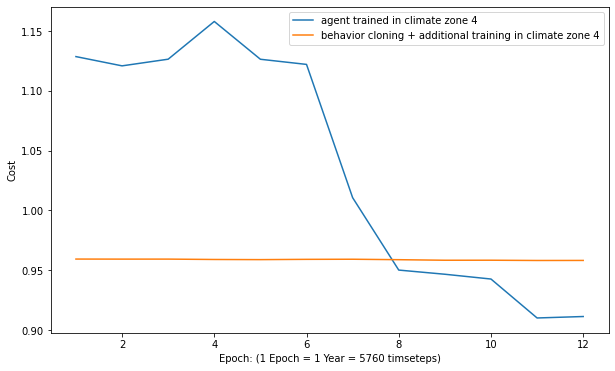
\includegraphics[width=\linewidth]{figures/bc_vs_sac.png}
    \caption{Comparison of training curves between SAC and BC}
    \label{fig:bc_vs_sac}
  \end{minipage}
  \hfill
  \begin{minipage}[b]{0.45\textwidth}
    \centering
    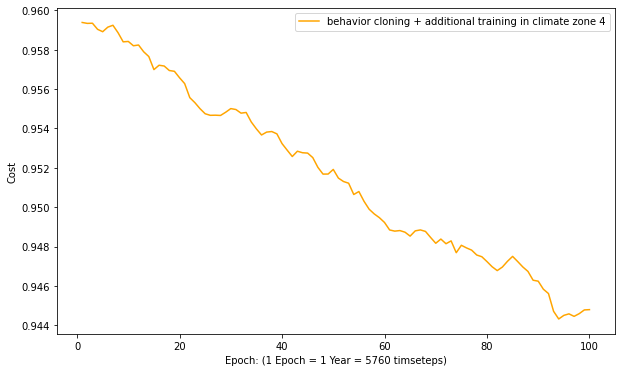
\includegraphics[width=\linewidth]{figures/bc_single.png}
    \caption{Enlarged view of training curve of behavior cloning}
    \label{fig:bc_single}
  \end{minipage}
\end{figure}

As an evaluation of this approach, it can generate better cost compared to SAC agent. However, it is fatal that the additional training is not efficient, and it takes a longer time to adapt to the environment. Behavior cloning can be used if we do not need to adapt to the environment and just imitate an external expert. In addition to the previous section, \ref{sec:TL}, we can conclude that both policy and value networks should be pre-trained on certain region, as its outperforms behavior cloning method. 

\section{Conclusion/Discussion}


\subsection{MAML}

The limitations of our method are in generalization and the policy's long training period. We have shown that policy does not do well on generalization over other regions, especially compared to the trained regions in the cost. Due to a lack of generalization, we might need to train the policy for each region separately. However, it takes at least ten years to train an adequate policy. To address this problem, we plan to incorporate Model-Agnostic Meta-Learning(MAML) algorithm, which will deal with over-fitting problems and decrease the policy's training period.\cite{finn2017modelagnostic} There are numerous interpretation of MAML. One of them is that the algorithm is designed to make the policy to learn shared components between different regions. It learns shared components by averaging different gradient descents updates from each region. In more detail, it will sample trajectories from each n sampled regions. It will update its parameters for n policies, copies of the original policy, using gradient descent. Using those n updated policies, it will sample another h trajectories. It will update the original policy by averaging those different gradient descents updates from h trajectories. In theory the learning of unique components will decrease from this average process. After learning shared components, we would have fine-tuning process, in which policy learns its unique components. Since the policy only has to learn the unique components after using MAML, the required training period will decrease, especially compared to learning from scratch. 
\newline
We did face some obstacles from implementing MAML into our environment. Most of the packages for MAML are for a single agent. However, our citylearn environment has multiple agents. Furthermore, we are interested in optimizing the policy in a competitive environment, so we also need to optimize other remaining policies to establish this environment. We thought our problem was similar to Gibbs sampling problem, a sampling problem for distributions that has a dependent relationship, as our optimizing agent also depends on other agents' policy. In this case, we cannot directly optimize or sample from a single agent or single parameter. Inspired by Gibbs sampling algorithm, we would iteratively update each policy, so each iteration the policy would be, in theory, optimized in a more competitive environment than previous iterations. The pseudocode for our algorithm is written in
\newline

\textbf{Algorithm\ref{algo:multi-maml}}. We are currently working on this problem. 

\begin{algorithm}
    \caption{Multi-agent MAML}
    \label{algo:multi-maml}
  \begin{algorithmic}[1]
    \REQUIRE $P(Z):$ distribution of zones
    \REQUIRE $\theta_{i}:$ policy for each building in the environment
    \REQUIRE $\alpha$, $\beta:$ step size parameter for update
    \WHILE{not done}
        \FOR{\textbf{all} $\theta_{i}$}
        \State sample batch of zones $Z_{j} \sim P(Z)$
            \FOR{\textbf{all} $Z_{j}$}
                \State Sample K trajectories $D = \{(x_{1}, a_{1}, ...x_{H})\}$ using $f_{\theta_{i}}$ in the environment with zone $Z_{j}$
                \State Evaluate $\nabla_{\theta_{i}}L_{Z_{j}}(f_{\theta_{i}})$ using $D$ and $L_{Z_{j}}$
                \State compute adapted parameters using gradient descent $\theta^{'}_{i,j} = \theta - \alpha \nabla_{\theta_{i}}L_{Z_{j}}(f_{\theta_{i}})$
                \State Sample trajectories $D^{'}_{j} = \{(x_{1}, a_{1}, ...x_{H})\}$ using $f_{\theta^{'}_{i,j}}$ in zone $Z_{j}$
            \ENDFOR
            \State Update $\theta_{i} = \theta_{i} -\beta \nabla_{\theta_{i}}\sum_{Z_{j} \sim P(Z)} L_{Z_{j}}(f_{\theta_{i,j}})$ using each $D^{'}_{j}$ and $L_{Z_{j}}$
        \ENDFOR
    \ENDWHILE
  \end{algorithmic}
\end{algorithm}

\subsection{Applicability}

There are some concerns about whether the trained policy could be applicable in real life. One of the concern is whether the simulation from the citylearn environment will be similar to what is actually happening in the real-life environment. For example, citylearn environment has only nine types of building. It is unlikely that those nine types of building will represent all different building types in real life. Furthermore, the citylearn environment assumes that nine types of building will be the same for different zones. However, each zone's building types should be different as they would be built differently in material and structure. For example, an architect from warmer zones will use other material compared to an architect from colder zones to account for climate and temperature. If there is such a difference, then buildings should generate different states if they have the same weather. Yet, such circumstances is not accounted in the citylearn environment. Therefore, we need to study further how climate affects architecture and apply it to citylearn to overcome this problem. 
\newline
Another concern is whether policy that had been optimized in the environment with nine buildings will generalize into the environment with at least more than 1000 buildings. Original scholars and we used an environment with only nine buildings due to computational cost. Optimization could be more complicated and different when the number of buildings increases in the environment. If this is the case, we might impose a bias into our policy, which might lead to worse outcome than training from scratch. To overcome this problem, we should also look into how we could generalize the policy when there are a different number of buildings in the environment. 


%\bibliographystyle{plain}
% citation: order of appearance
\bibliographystyle{unsrt}
\bibliography{References.bib}

\end{document}